\documentclass[../../statistical_learning_notes.tex]{subfiles}
\begin{document}
%%%%%%%%%%%%%%%%%%%%%%%%%%%%%%%%%%%%%%%%%%%%%%%%%%%%%%%%%%%%%%%%%%%%%%%%%%%
\section{Sampling from Distributions}
\subsection{Rejection Sampling}
Consider a probability distribution $p(x)$ that we want to sample from, and suppose there is another distribution $q(x)$ such that $p(x) \leq Mq(x)$ where $M$ is a constant scalar. Assume that $q$ is a distribution from which we can easily sample. Then to sample from $p(x)$
\begin{enumerate}
    \item Sample a point $x_{0}$ from $q(x)$
    \item Sample a point $u$ from $Uniform(0,Mq(x_{0}))$
    \item Accept $x_{0}$ with probability $\frac{p(x_{0})}{Mq(x_{0})}$ if $u \leq p(x_{0})$
\end{enumerate}

The scheme works because any point we are accepting lies inside the curve $p(x)$. Also, on average, we will get $1$ accepted point for every $M$ samples because the total points generated cover the area under $q(x)$ while the accepted ones cover the area under $Mq(x)$. The total points accepted are simply the ratios of area under $p(x)$ and $M(q(x)$.\newline

The technique works equally well if we know the distribution only upto a normalization constant
\begin{gather*}
    \frac{\tilde{p}(x)}{Z} \leq Mq(x) \implies \tilde{p}(x) \leq M^{\prime}q(x), \; M^{\prime} = ZM
\end{gather*}

\begin{figure}[h]
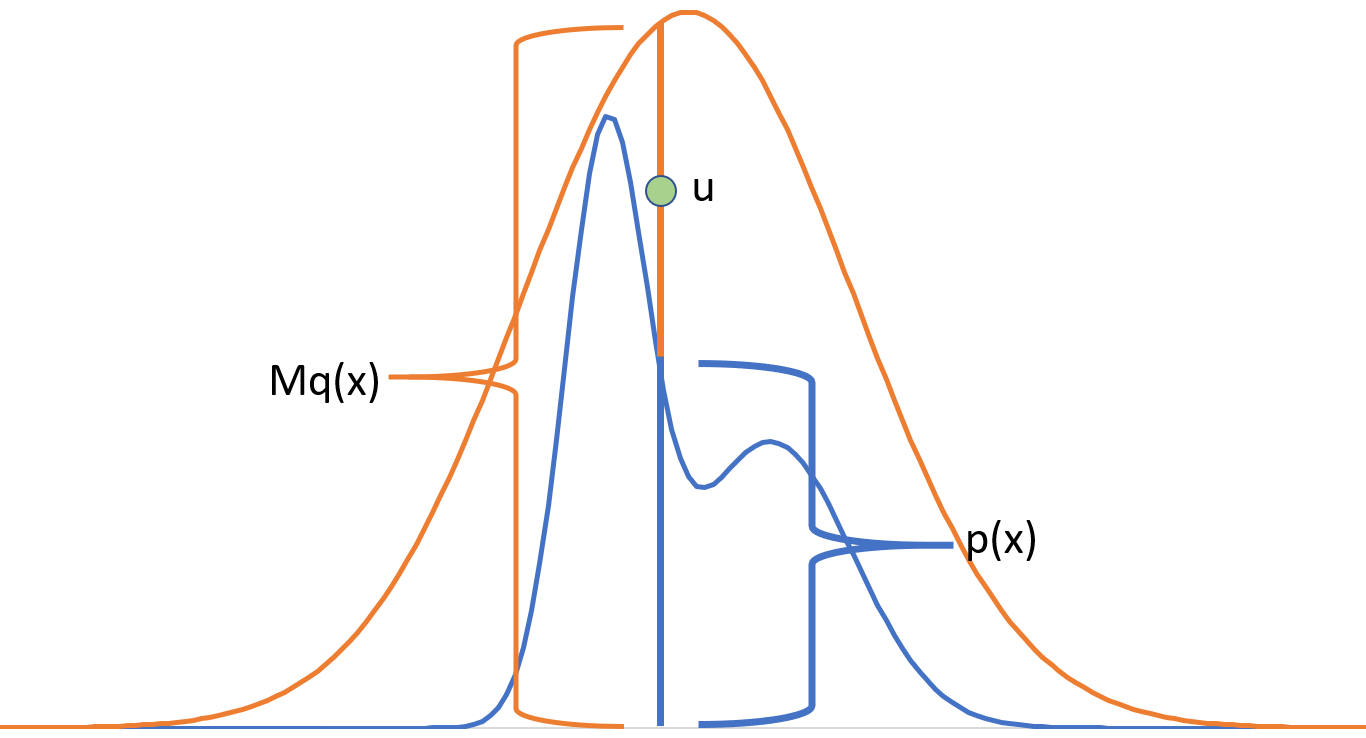
\includegraphics[scale=0.3]{sampling_1}
\centering
\caption{Rejection Sampling: $u$ is selected with probability $p(x)/Mq(x)$}
\label{fig:sampling_1} %\ref{fig:sampling_1}
\end{figure}
\end{document}